\section{The $t$ distribution for the difference of two means}

It is useful to be able to compare two means. For instance, a teacher might like to test the notion that two versions of an exam were equally difficult. She could do so by randomly assigning each version to students. If she found that the average scores on the exams were so different that we cannot write it off as chance, then she may want to award extra points to students who took the more difficult exam.

In a medical context, we might investigate whether embryonic stem cells (ESCs) can improve heart pumping capacity in individuals who have suffered a heart attack. We could look for evidence of greater heart health in the ESC group against a control group.

The ability to make conclusions about a difference in two means, $\mu_1 - \mu_2$, is often useful. If the sample sizes are small and the data are nearly normal, the $t$ distribution can be applied to the sample difference in means, $\bar{x}_1 - \bar{x}_2$, to make inference about the difference in population means.

\subsection{Sampling distributions for the difference in two means}

In the example of two exam versions, the teacher would like to evaluate whether there is convincing evidence that the difference in average scores is not due to chance.

It will be useful to extend the $t$ distribution method from Section~\ref{oneSampleMeansWithTDistribution} to apply to a new point estimate:
\begin{eqnarray*}
\bar{x}_1 - \bar{x}_2
\end{eqnarray*}
Just as we did in Section~\textbf{\color{red}5.2}, we verify conditions for each sample separately and then verify that the samples are also independent. For instance, if the teacher believes students in her class are independent, the exam scores are nearly normal, and the students taking each version of the exam were independent, then we can use the $t$ distribution for the sampling distribution of the point estimate, $\bar{x}_{1} - \bar{x}_{2}$.

The formula for the standard error of $\bar{x}_{1} - \bar{x}_{2}$, introduced in Section~\textbf{\color{red}5.2},
remains useful for small samples:
\begin{eqnarray}
SE_{\bar{x}_1 - \bar{x}_2}
	= \sqrt{SE_{\bar{x}_1}^2 + SE_{\bar{x}_2}^2}
	 = \sqrt{\frac{s_1^2}{n_1} + \frac{s_2^2}{n_2}} \label{seOfDiffOfTwoMeansInTDistSection}
\end{eqnarray}
Because we will use the $t$ distribution, we will need to identify the appropriate degrees of freedom. This can be done using computer software. An alternative technique is to use the smaller of $n_1 - 1$ and $n_2 - 1$, which is the method we will apply in the examples and exercises\footnote{This technique for degrees of freedom is conservative with respect to a Type 1 Error; it is more difficult to reject the null hypothesis using this $df$ method.}. 

\begin{termBox}{\tBoxTitle{Using the $t$ distribution for a difference in means}
The $t$ distribution can be used for the (standardized) difference of two means if (1) each sample meets the conditions for the $t$ distribution and (2) the samples are independent. We estimate the standard error of the difference of two means using Equation~(\ref{seOfDiffOfTwoMeansInTDistSection}).}
\end{termBox}

%In this section, we apply the same $t$ distribution methods of Section~\ref{oneSampleMeansWithTDistribution} to the point estimate of the difference in means: $\bar{x}_1 - \bar{x}_2$.

\subsection{Two sample $t$ test}
%Do not include the test with pooled standard deviations are grouped but mention it as one method that is discussed in other books.% (I consider this to be a poor test -- if the sd's are remotely similar then the result will be basically the same as the sd's are not assumed to be the same... seems like a big assumption that can results in too many problems with almost no benefits.)

%Two versions of an exam were given out to students to reduce cheating. However, when the professor examined the average scores on the two exams, she saw that they were different. 
Summary statistics for each exam version are shown in Table~\ref{summaryStatsForTwoVersionsOfExams}. The teacher would like to evaluate whether this difference is so large that it provides convincing evidence that Version B was more difficult (on average) than Version A. 

\begin{table}[hht]
\centering
\begin{tabular}{l rrrrr}
\hline
Version\hspace{2mm}	& $n$	& $\bar{x}$	& $s$	& min	& max  \\
\hline
A		& 30		& 79.4		& 14 	& 45		& 100 \\
B		& 27		& 74.1		& 20		& 32		& 100 \\
\hline
\end{tabular}
\caption{Summary statistics of scores for each exam version.}
\label{summaryStatsForTwoVersionsOfExams}
\end{table}

\begin{exercise} \label{htSetupForEvaluatingTwoExamVersions}
Construct a two-sided hypothesis test to evaluate whether the observed difference in sample means, $\bar{x}_A - \bar{x}_B=5.3$, might be due to chance. Answer in the footnote\footnote{Because the professor did not expect one exam to be more difficult prior to examining the test results, she should use a two-sided hypothesis test. $H_0$: the exams are equally difficult, on average. $\mu_A - \mu_B = 0$. $H_A$: one exam was more difficult than the other, on average. $\mu_A - \mu_B \neq 0$.}.
\end{exercise}

\begin{exercise} \label{conditionsForTDistForEvaluatingTwoExamVersions}
To evaluate the hypotheses in Exercise~\exer{htSetupForEvaluatingTwoExamVersions} using the $t$ distribution, we must first verify assumptions. (a) Does it seem reasonable that the scores are independent? (b) What about the normality condition for each group? (c) Do you think each group would be independent? Answer in the footnote\footnote{(a) It is probably reasonable to conclude the scores are independent. (b) The summary statistics suggest the data are roughly symmetric about the mean, and it doesn't seem unreasonable to suggest the data might be normal. (c) It seems reasonable to suppose that the samples are independent since the exams were handed out randomly.}.
\end{exercise}

After verifying the conditions for each sample and confirming the samples are independent of each other, we are ready to conduct the test using the $t$ distribution. In this case, we are estimating the true difference in average test scores using the sample data, so the point estimate is $\bar{x}_A - \bar{x}_B = 5.3$. The standard error of the estimate can be calculated using Equation~(\ref{seOfDiffOfTwoMeansInTDistSection}):
\begin{eqnarray*}
SE = \sqrt{\frac{s_A^2}{n_A} + \frac{s_B^2}{n_B}} = \sqrt{\frac{14^2}{30} + \frac{20^2}{27}} = 4.62
\end{eqnarray*}
Finally, we construct the test statistic:
\begin{eqnarray*}
T = \frac{\text{point estimate} - \text{null value}}{SE} = \frac{(79.4-74.1) - 0}{4.62} = 1.15
\end{eqnarray*}
If we have a computer handy, we can identify the degrees of freedom as 45.97. Otherwise we use the smaller of $n_1-1$ and $n_2-1$: $df=26$. 

\begin{figure}
\centering
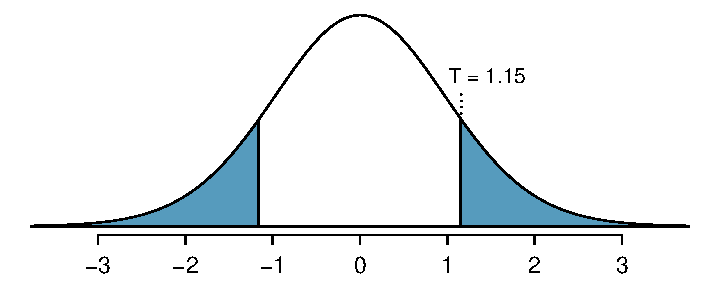
\includegraphics[width=0.65\textwidth]{06/figures/pValueOfTwoTailAreaOfExamVersionsWhereDFIs26/pValueOfTwoTailAreaOfExamVersionsWhereDFIs26}
\caption{The $t$ distribution with 26 degrees of freedom. The shaded right tail represents values with $T \geq 1.15$. Because it is a two-sided test, we also shade the corresponding lower tail.}
\label{pValueOfTwoTailAreaOfExamVersionsWhereDFIs26}
\end{figure}

\begin{exercise} \label{computeTwoTailAreaOfExamVersionsWhereDFIs26}
Identify the p-value, shown in Figure~\ref{pValueOfTwoTailAreaOfExamVersionsWhereDFIs26}. Use $df=26$. Answer in the footnote\footnote{We examine row $df=26$ in the $t$ table. Because this value is smaller than the value in the left column, the p-value is at least 0.200 (two tails!). Because the p-value is so large, we do not reject the null hypothesis. That is, the data do not convincingly show that one exam version is more difficult than the other, and the teacher is not convinced that she should add points to the Version B exam scores.}.
\end{exercise}

In Exercise~\exer{computeTwoTailAreaOfExamVersionsWhereDFIs26}, we could have used $df=45.97$. However, this value is not listed in the table. In such cases, we use the next lower degrees of freedom (unless the computer also provides the p-value). For example, we could have used $df=45$ but not $df=46$. 

Do embryonic stem cells (ESCs) help improve heart function following a heart attack? Table~\ref{summaryStatsForSheepHeartDataWhoReceivedMiceESCs} contains summary statistics for an experiment to test ESCs in sheep that had a heart attack. Each of these sheep was randomly assigned to the ESC or control group, and the change in their hearts' pumping capacity was measured. A positive value generally corresponds to increased pumping capacity, which suggests a stronger recovery. We will consider this study in the exercises and examples below.

\begin{exercise} \label{exerciseToEvaluteWhetherESCsAreHelpfulInImprovingHeartFunctionInSheep}
Set up hypotheses that will be used to test whether there is convincing evidence that ESCs actually increase the amount of blood the heart pumps. Answer in the footnote\footnote{We first setup the hypotheses:
\begin{itemize}
\item[$H_0$:] The stem cells do not improve heart pumping function. $\mu_{esc} - \mu_{control} = 0$.
\item[$H_A$:] The stem cells do improve heart pumping function. $\mu_{esc} - \mu_{control} > 0$.
\end{itemize}
Before we move on, we must first verify that the $t$ distribution method can be applied. Because the sheep were randomly assigned their treatment and, presumably, were kept separate from one another, the independence assumption is verified for each sample as well as for between samples. The data are very limited, so we can only check for obvious outliers in the raw data in Figure~\ref{stemCellTherapyForHearts}. Since the distributions are (very) roughly symmetric, we will assume the normality condition is acceptable. Because the conditions are satisfied, we can apply the $t$ distribution.}.
\end{exercise}

\begin{table}
\centering
\begin{tabular}{l rrrrr}
\hline
\hspace{10mm}	& $n$	& $\bar{x}$	& $s$  	 \\
\hline
ESCs		& 9		& 3.50		& 5.17  	\\
control		& 9		& -4.33		& 2.76  	 \\
\hline
\end{tabular}
\caption{Summary statistics of scores, split by exam version.}
\label{summaryStatsForSheepHeartDataWhoReceivedMiceESCs}
\end{table}

\begin{figure}
\centering
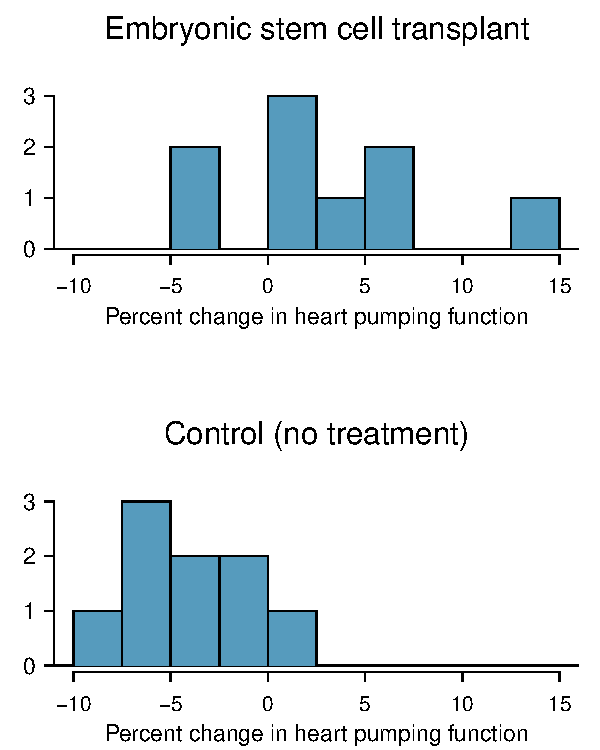
\includegraphics[width=0.6\textwidth]{06/figures/stemCellTherapyForHearts/stemCellTherapyForHearts}
\caption{Histograms for both the embryonic stem cell group and the control group. Higher values are associated with greater improvement.}
\label{stemCellTherapyForHearts}
\end{figure}

\begin{example}{The raw data from the ESC experiment described in Exercise~\ref{exerciseToEvaluteWhetherESCsAreHelpfulInImprovingHeartFunctionInSheep} may be viewed in Figure~\ref{stemCellTherapyForHearts}. Using 8 degrees of freedom for the $t$ distribution, evaluate the hypotheses.}
We first compute the point estimate of the difference along with the standard error:
\begin{align*}
& \bar{x}_{esc} - \bar{x}_{control} = 7.88 \\
& SE = \sqrt{\frac{5.17^2}{9} + \frac{2.76^2}{9}} = 1.95
\end{align*}
The p-value is depicted as the shaded right tail in Figure~\ref{stemCellTherapyForHeartsPValue}, and the test statistic is computed as follows:
$$T = \frac{7.88 - 0}{1.95} = 4.03$$
We use the smaller of $n_1-1$ and $n_2-1$ (each are the same) for the degrees of freedom: $df=8$. Finally, we look for $T=4.03$ in the $t$ table; it falls to the right of the last column, so the p-value is smaller than 0.005 (one tail!). Because the p-value is less than 0.005 and therefore also smaller than 0.05, we reject the null hypothesis. The data provide convincing evidence that embryonic stem cells improve the heart's pumping function in sheep that have suffered a heart attack.
\end{example}

\begin{figure}
\centering
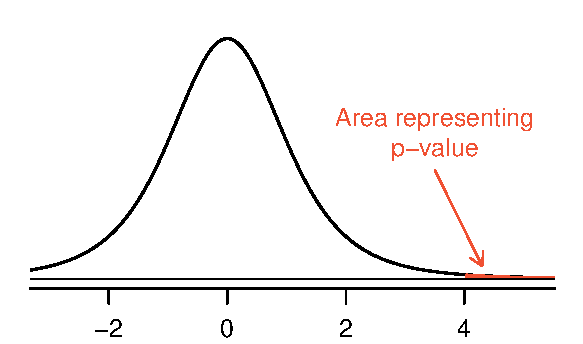
\includegraphics[width=0.6\textwidth]{06/figures/stemCellTherapyForHeartsPValue/stemCellTherapyForHeartsPValue}
\caption{Distribution of the sample difference of the mean improvements if the null hypothesis was true. The shaded area represents the p-value.}
\label{stemCellTherapyForHeartsPValue}
\end{figure}

\subsection{Two sample $t$ confidence interval}

Based on the results of Exercise~\exer{exerciseToEvaluteWhetherESCsAreHelpfulInImprovingHeartFunctionInSheep}, you found significant evidence that ESCs actually help improve the pumping function of the heart. But how large is this improvement? To answer this question, we can use a confidence interval. 

\begin{exercise}
In Exercise~\exer{exerciseToEvaluteWhetherESCsAreHelpfulInImprovingHeartFunctionInSheep}, you found that the point estimate, $\bar{x}_{esc} - \bar{x}_{control} = 7.88$, has a standard error of 1.95. Using $df=8$, create a 99\% confidence interval for the improvement due to ESCs. Answer in the footnote\footnote{We know the point estimate, 7.88, and the standard error, 1.95. We also verified the conditions for using the $t$ distribution in Exercise~\exer{exerciseToEvaluteWhetherESCsAreHelpfulInImprovingHeartFunctionInSheep}. Thus, we only need identify $t^{\star}_8$ to create a 99\% confidence interval: $t^{\star}_{8} = 3.36$. Thus, the 99\% confidence interval for the improvement from ESCs is given by $$7.88 \pm 3.36*1.95 \quad\to\quad (1.33, 14.43)$$ That is, we are 99\% confident that the true improvement in heart pumping function is somewhere between 1.33\% and 14.43\%.}.
\end{exercise}

\subsection{Pooled standard deviation estimate (special topic)}
\label{pooledStandardDeviations}

Occasionally, two populations will have standard deviations that are so similar, that they can be treated as identical. For example, historical data or a well-understood biological mechanism may justify this strong assumption. In such cases, we can make our $t$ distribution approach slightly more precise by using a pooled standard deviation.

The \term{pooled standard deviation} of two groups is a way to use data from both samples to better estimate the standard deviation and standard error. If $s_1^{}$ and $s_2^{}$ are the standard deviations of groups 1 and 2 and there are good reasons to believe that the population standard deviations are equal, then we can obtain an improved estimate of the group variances by pooling their data:
\begin{align*}
s_{pooled}^2 = \frac{s_1^2*(n_1-1) + s_2^2*(n_2-1)}{n_1 + n_2 - 2}
\end{align*}
where $n_1$ and $n_2$ are the sample sizes, as before. To utilize this new statistic, we substitute $s_{pooled}^2$ in place of $s_1^2$ and $s_2^2$ in the standard error formula, and we use an updated formula for the degrees of freedom:
\begin{align*}
df = n_1 + n_2 - 2
\end{align*}

The benefits of pooling the standard deviation are realized through obtaining a better estimate of the population standard deviations and using a larger degrees of freedom parameter for the $t$ distribution. Both of these changes may permit a better model of the sampling distribution of $\bar{x}_1^2 - \bar{x}_2^2$.

\begin{caution}
{Pooling standard deviations should be done only after careful research}
{A pooled standard deviation is only appropriate when background research indicates the population standard deviations are nearly equal. When the sample size is large and the condition may be adequately checked with data, the benefits of pooling the standard deviations greatly diminishes.}
\end{caution}

%As a general rule of thumb, we advise implementing the unequal standard deviation approach promoted earlier in this section unless there is strong reason to believe the standard deviations are equal. 
%However, we will find that pooled standard deviations are useful to a commonly used technique in Chapter~\ref{multipleRegressionAndANOVA} called analysis of variance (ANOVA).


%As a general rule of thumb, we advise against pooling standard deviations for the two-sample mean test due to the difficulty in. Verifying the assumption that the standard deviations are equal is difficult without a large sample, and in such cases, there is virtually no difference between using the standard estimates of standard deviation and using the pooled approach.

